\documentclass[tikz,border=2pt]{standalone}
\usepackage[T1]{fontenc}
\usepackage{tgheros}
\renewcommand{\familydefault}{\sfdefault}
\usetikzlibrary{arrows.meta,fit,positioning}

\definecolor{dirblue}{HTML}{9FC5E8}
\definecolor{filegreen}{HTML}{B6D7A8}
\definecolor{packageblue}{HTML}{3D85C6}

\begin{document}
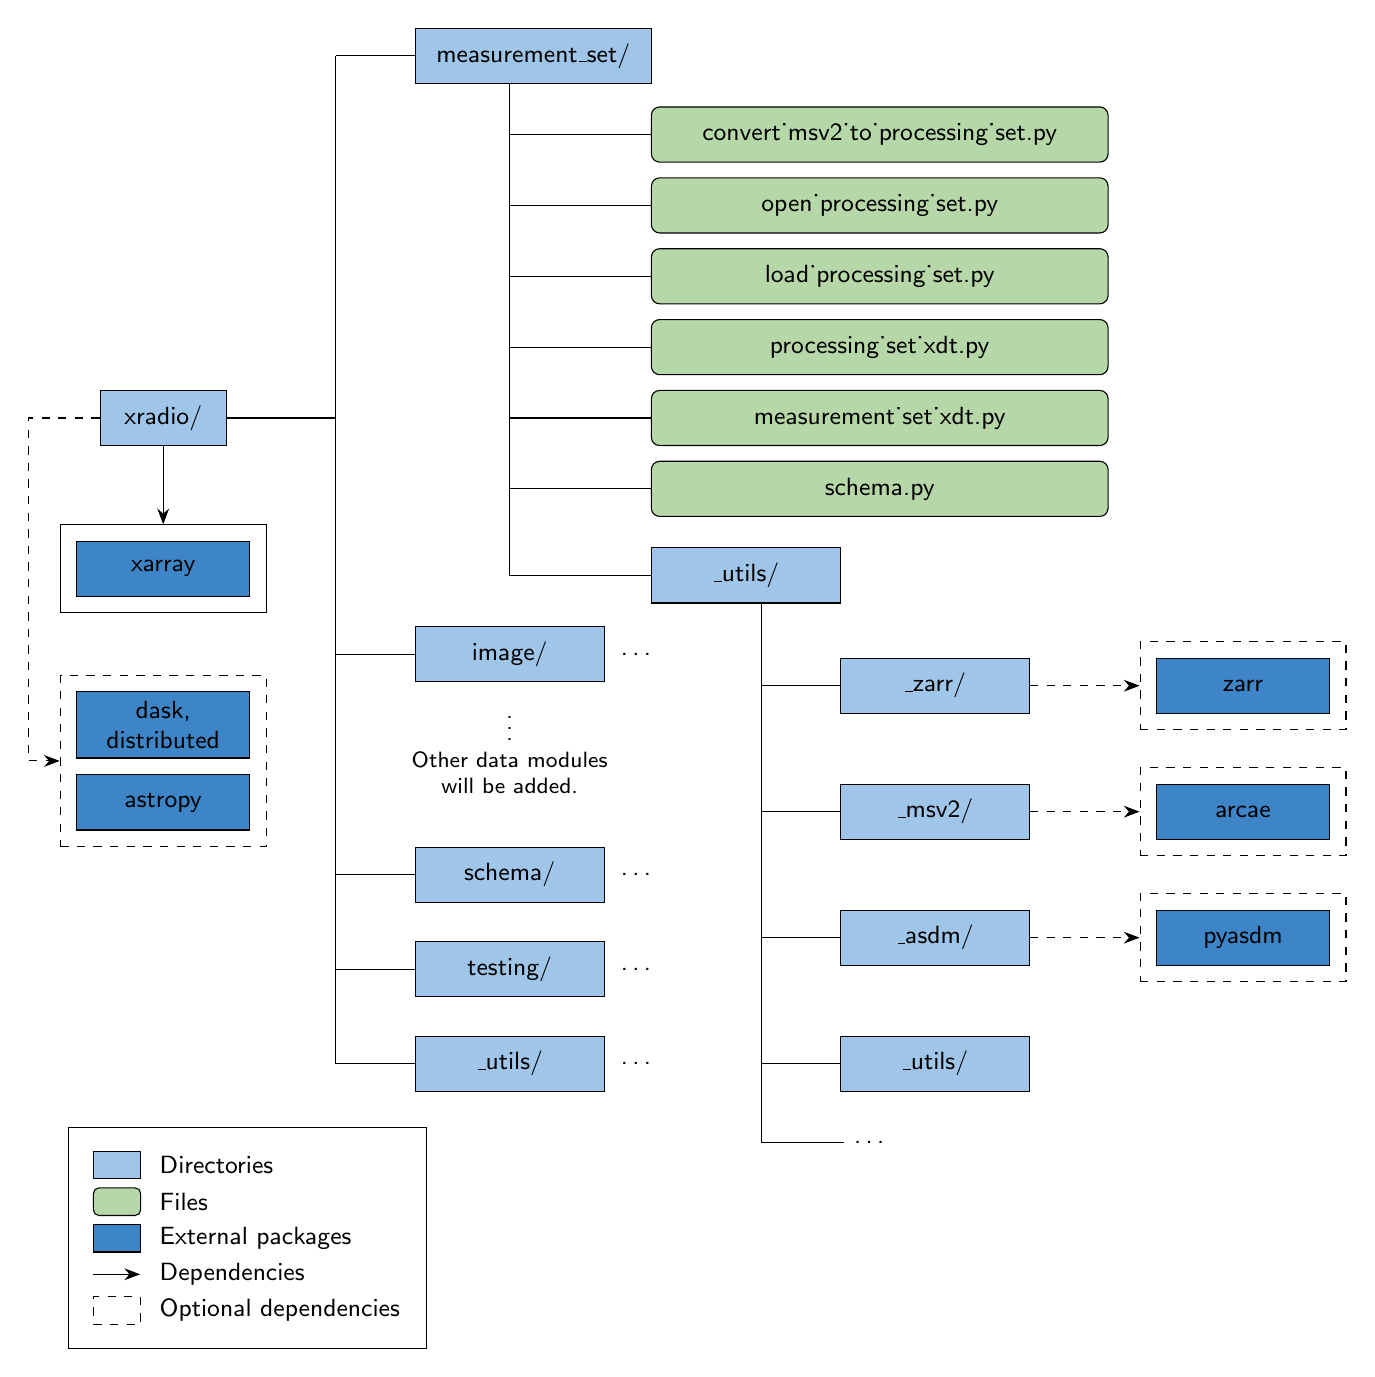
\begin{tikzpicture}[
    font=\small,
    dir/.style={draw, fill=dirblue, minimum height=7mm, minimum width=2.4cm,
      anchor=west},
    file/.style={draw, fill=filegreen, rounded corners=3pt, minimum height=7mm,
      minimum width=5.8cm, anchor=west},
    package/.style={draw, fill=packageblue, minimum height=7mm,
      minimum width=2.2cm, align=center},
    group/.style={draw, inner sep=2mm},
    optional/.style={group, dashed},
    depends/.style={-{Stealth[length=2mm]}},
    optional depends/.style={depends, dashed},
    more/.style={right=2mm of #1, anchor=west, inner sep=0pt},
  ]
  % xradio/ and its dependencies
  \node[dir, minimum width=1.6cm] (xradio) at (0, -4.6) {xradio/};
  \node[package, below=1.2cm of xradio] (xarray) {xarray};
  \node[group, fit=(xarray)] (required) {};
  \node[package, below=1.2cm of xarray] (dask) {dask,\\ distributed};
  \node[package, below=2mm of dask] (astropy) {astropy};
  \node[optional, fit=(dask) (astropy)] (extras) {};
  \draw[depends] (xradio) -- (required);
  \draw[optional depends] (xradio.west) -| ([xshift=-4mm]extras.west) -- (extras.west);

  % sub-packages
  \coordinate (trunk) at (3, 0);
  \node[dir, minimum width=3cm] (ms) at (4, 0) {measurement\_set/};
  \node[dir] (image) at (4, -7.6) {image/};
  \node[more=image] {\dots};
  \node[below=1mm of image, align=center, font=\footnotesize]
    {\vdots\\ Other data modules\\ will be added.};
  \node[dir] (schema) at (4, -10.4) {schema/};
  \node[more=schema] {\dots};
  \node[dir] (testing) at (4, -11.6) {testing/};
  \node[more=testing] {\dots};
  \node[dir] (utils) at (4, -12.8) {\_utils/};
  \node[more=utils] {\dots};
  \draw (xradio.east) -- (trunk |- xradio);
  \draw (trunk) -- (trunk |- utils);
  \foreach \n in {ms, image, schema, testing, utils}
    \draw (trunk |- \n) -- (\n);

  % measurement_set/
  \coordinate (ms trunk) at ([xshift=1.2cm]ms.south west);
  \foreach \f [count=\i] in {convert_msv2_to_processing_set.py,
      open_processing_set.py, load_processing_set.py, processing_set_xdt.py,
      measurement_set_xdt.py, schema.py} {
    \node[file] (file\i) at (7, -0.9 * \i - 0.1) {\detokenize\expandafter{\f}};
    \draw (ms trunk |- file\i) -- (file\i);
  }
  \node[dir] (ms utils) at (7, -6.6) {\_utils/};
  \draw (ms trunk) -- (ms trunk |- ms utils) -- (ms utils);

  % measurement_set/_utils/
  \coordinate (utils trunk) at ([xshift=1.4cm]ms utils.south west);
  \node[dir] (zarr) at (9.4, -8) {\_zarr/};
  \node[dir] (msv2) at (9.4, -9.6) {\_msv2/};
  \node[dir] (asdm) at (9.4, -11.2) {\_asdm/};
  \node[dir] (ms utils utils) at (9.4, -12.8) {\_utils/};
  \node (ms utils more) at (9.8, -13.8) {\dots};
  \draw (utils trunk) -- (utils trunk |- ms utils more.west) -- (ms utils more);
  \foreach \n in {zarr, msv2, asdm, ms utils utils}
    \draw (utils trunk |- \n) -- (\n);
  \foreach \n/\p in {zarr/zarr, msv2/arcae, asdm/pyasdm} {
    \node[package, right=1.6cm of \n] (\n package) {\p};
    \node[optional, fit=(\n package)] (\n group) {};
    \draw[optional depends] (\n) -- (\n group);
  }

  % legend
  \matrix[draw, anchor=north west, column sep=2mm, row sep=1mm,
      inner sep=3mm, nodes={anchor=west, inner sep=1pt}] at (-0.4, -13.6) {
    \node[draw, fill=dirblue, minimum width=6mm, minimum height=3.5mm] {}; &
      \node {Directories}; \\
    \node[draw, fill=filegreen, rounded corners=2pt, minimum width=6mm,
      minimum height=3.5mm] {}; & \node {Files}; \\
    \node[draw, fill=packageblue, minimum width=6mm, minimum height=3.5mm] {}; &
      \node {External packages}; \\
    \draw[depends] (0, 0) -- (6mm, 0); & \node {Dependencies}; \\
    \node[draw, dashed, minimum width=6mm, minimum height=3.5mm] {}; &
      \node {Optional dependencies}; \\
  };
\end{tikzpicture}
\end{document}
